\chapter{ソートアルゴリズム - Sorting}

\index{ソートアルゴリズム - sorting}

\key{ソートアルゴリズム - Sorting}
は典型的なアルゴリズムの問題です。
多くのアルゴリズムはソートを使用しています。
要素がソートされた順番になっていれば、データ処理が容易になる問題が多いからです。

例えば、「配列の中に同じ要素が2つあるか」という問題はソートを使えば簡単に解くことができます。
ソートされている配列に2つの等しい要素があれば隣り合っているので簡単に見つけることができます。
また、「配列の中で最も頻度の高い要素は何か」という問題も同様に解くことができます。

ソートには多くのアルゴリズムがあり、様々なアルゴリズムを検討する良い例にもなっています。
一般的に用いられるソートアルゴリズム は $O(n \log n)$時間で動作し、
ソートをサブルーチンとして使用する多くのアルゴリズムもこの時間複雑性を持ちます。

\section{ソートの理論 - Sorting theory}

ソートの最も基本的な問題は次の通りです。
\begin{framed}
\noindent
 n個の要素を含む配列が与えられたとき、要素を昇順に並べ替えてください。
\end{framed}
\noindent
\begin{center}
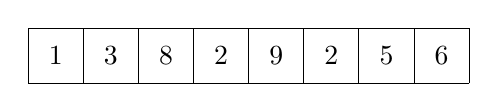
\begin{tikzpicture}[scale=0.7]
\draw (0,0) grid (8,1);
\node at (0.5,0.5) {$1$};
\node at (1.5,0.5) {$3$};
\node at (2.5,0.5) {$8$};
\node at (3.5,0.5) {$2$};
\node at (4.5,0.5) {$9$};
\node at (5.5,0.5) {$2$};
\node at (6.5,0.5) {$5$};
\node at (7.5,0.5) {$6$};
\end{tikzpicture}
\end{center}
この配列を次のように操作します。
\begin{center}
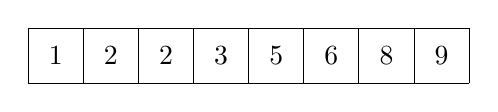
\begin{tikzpicture}[scale=0.7]
\draw (0,0) grid (8,1);
\node at (0.5,0.5) {$1$};
\node at (1.5,0.5) {$2$};
\node at (2.5,0.5) {$2$};
\node at (3.5,0.5) {$3$};
\node at (4.5,0.5) {$5$};
\node at (5.5,0.5) {$6$};
\node at (6.5,0.5) {$8$};
\node at (7.5,0.5) {$9$};
\end{tikzpicture}
\end{center}

\subsubsection{$O(n^2)$ アルゴリズム}

\index{バブルソート - bubble sort}
配列をソートするための最も簡単なアルゴリズムは、$O(n^2)$ 時間で動作します。
このアルゴリズムはシンプルに記述でき2つの入れ子ループで構成されます。
有名な $O(n^2)$ のソートアルゴリズムを紹介します。
\key{バブルソート - bubble sort}は各要素をその名の通りバブル(浮き上げ)させます。

バブルソートは$n$回のラウンドで構成されて各ラウンドでは配列の要素を繰り返し処理します。
連続する2つの要素で順序が正しくないペアが見つかるとそれを交換します。
このアルゴリズムは以下のように実装することができます。

\begin{lstlisting}
for (int i = 0; i < n; i++) {
    for (int j = 0; j < n-1; j++) {
        if (array[j] > array[j+1]) {
            swap(array[j],array[j+1]);
        }
    }
}
\end{lstlisting}

最初のラウンドのあと、最大の値は正しい場所にあることが保証されます。
そして、$k$ラウンドの後には、上から$k$個の要素は正しい位置にあることが保証されます。
つまり、$n$ラウンド後にはソートが完了します。

\begin{center}
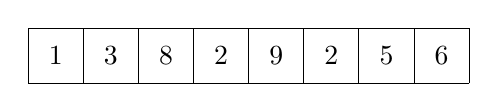
\begin{tikzpicture}[scale=0.7]
\draw (0,0) grid (8,1);

\node at (0.5,0.5) {$1$};
\node at (1.5,0.5) {$3$};
\node at (2.5,0.5) {$8$};
\node at (3.5,0.5) {$2$};
\node at (4.5,0.5) {$9$};
\node at (5.5,0.5) {$2$};
\node at (6.5,0.5) {$5$};
\node at (7.5,0.5) {$6$};
\end{tikzpicture}
\end{center}

\noindent
この時の最初のラウンドを見てみます。

\begin{center}
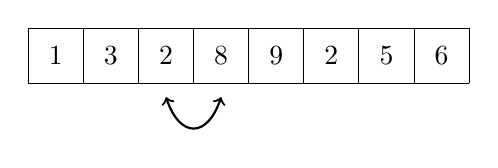
\begin{tikzpicture}[scale=0.7]
\draw (0,0) grid (8,1);
\node at (0.5,0.5) {$1$};
\node at (1.5,0.5) {$3$};
\node at (2.5,0.5) {$2$};
\node at (3.5,0.5) {$8$};
\node at (4.5,0.5) {$9$};
\node at (5.5,0.5) {$2$};
\node at (6.5,0.5) {$5$};
\node at (7.5,0.5) {$6$};

\draw[thick,<->] (3.5,-0.25) .. controls (3.25,-1.00) and (2.75,-1.00) .. (2.5,-0.25);
\end{tikzpicture}
\end{center}

\begin{center}
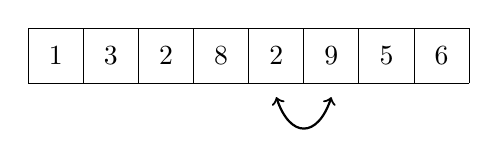
\begin{tikzpicture}[scale=0.7]
\draw (0,0) grid (8,1);
\node at (0.5,0.5) {$1$};
\node at (1.5,0.5) {$3$};
\node at (2.5,0.5) {$2$};
\node at (3.5,0.5) {$8$};
\node at (4.5,0.5) {$2$};
\node at (5.5,0.5) {$9$};
\node at (6.5,0.5) {$5$};
\node at (7.5,0.5) {$6$};

\draw[thick,<->] (5.5,-0.25) .. controls (5.25,-1.00) and (4.75,-1.00) .. (4.5,-0.25);
\end{tikzpicture}
\end{center}

\begin{center}
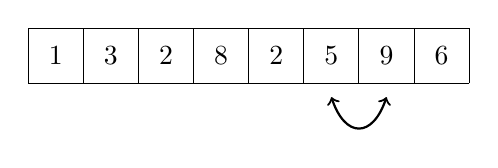
\begin{tikzpicture}[scale=0.7]
\draw (0,0) grid (8,1);
\node at (0.5,0.5) {$1$};
\node at (1.5,0.5) {$3$};
\node at (2.5,0.5) {$2$};
\node at (3.5,0.5) {$8$};
\node at (4.5,0.5) {$2$};
\node at (5.5,0.5) {$5$};
\node at (6.5,0.5) {$9$};
\node at (7.5,0.5) {$6$};

\draw[thick,<->] (6.5,-0.25) .. controls (6.25,-1.00) and (5.75,-1.00) .. (5.5,-0.25);
\end{tikzpicture}
\end{center}

\begin{center}
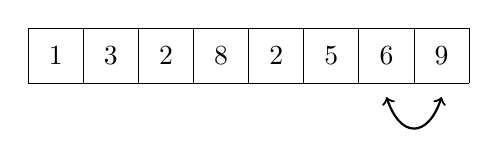
\begin{tikzpicture}[scale=0.7]
\draw (0,0) grid (8,1);
\node at (0.5,0.5) {$1$};
\node at (1.5,0.5) {$3$};
\node at (2.5,0.5) {$2$};
\node at (3.5,0.5) {$8$};
\node at (4.5,0.5) {$2$};
\node at (5.5,0.5) {$5$};
\node at (6.5,0.5) {$6$};
\node at (7.5,0.5) {$9$};

\draw[thick,<->] (7.5,-0.25) .. controls (7.25,-1.00) and (6.75,-1.00) .. (6.5,-0.25);
\end{tikzpicture}
\end{center}

\subsubsection{転置 - Inversions}

\index{転置 - inversion}

バブルソートは、配列中の連続した要素を常に入れ替えるソートアルゴリズムの一例です。
このようなアルゴリズムの時間計算量は常に$O(n^2)$となります。
なぜなら,最悪の場合,配列をソートするために $O(n^2)$のスワップが必要になるからです。

ソートアルゴリズムを解析する際に有用な概念に\key{転置 - inversion}があります。
$a<b$かつ$\texttt{array}[a]>\texttt{array}[b]$であるような要素の数を示します。
つまり、ソートされている順番に対して誤っているペアの数ともいえます。
\begin{center}
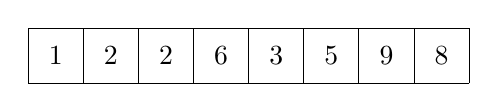
\begin{tikzpicture}[scale=0.7]
\draw (0,0) grid (8,1);
\node at (0.5,0.5) {$1$};
\node at (1.5,0.5) {$2$};
\node at (2.5,0.5) {$2$};
\node at (3.5,0.5) {$6$};
\node at (4.5,0.5) {$3$};
\node at (5.5,0.5) {$5$};
\node at (6.5,0.5) {$9$};
\node at (7.5,0.5) {$8$};
\end{tikzpicture}
\end{center}
を考えると3つの転置があります。$(6,3)$, $(6,5)$ , $(9,8)$の値のペアです。
反転の数は,配列の並べ替えにどれだけの作業が必要かを示します。
転置がないとき、配列は完全にソートされています。
一方,配列の要素が逆順(訳註:つまり降順)の場合に転地の数は最大となります.
\[1+2+\cdots+(n-1)=\frac{n(n-1)}{2} = O(n^2)\]


隣り合う順序を入れ替えると配列からちょうど1つの反転だけが削除されます。
つまり、ソートアルゴリズムが隣り合う要素の入れ替えしかできない場合に各入れ替えは最大でも1つの反転しか取り除けないため、
アルゴリズムは少なくとも$O(n^2)$です。

\subsubsection{$O(n \log n)$ アルゴリズム}

\index{マージソート - merge sort}

連続した要素の入れ替えに限らないアルゴリズムを用いれば$O(n \log n)$で効率的に配列をソートすることが可能です。
そのようなアルゴリズムの1つが 、再帰に基づくマージソート
\footnote{According to \cite{knu983},merge sort was invented by J. von Neumann in 1945.}
です。

マージソートは部分配列\texttt{array}$[a \ldots b]$に対して以下のような操作を行います。
\begin{enumerate}
\item $a=b$ならソートされているので何もしない
\item 中間のインデックスを計算する $k=\lfloor (a+b)/2 \rfloor$
\item 再帰的に \texttt{array}$[a \ldots k]$をソートする
\item 再帰的に \texttt{array}$[k+1 \ldots b]$をソートする
\item ソートされた\texttt{array}$[a \ldots k]$ と
\texttt{array}$[k+1 \ldots b]$ を \emph{マージ - Merge} し、
ソートされた配列\texttt{array}$[a \ldots b]$を作る
\end{enumerate}

マージソートは各ステップで部分配列のサイズを半分にすることで効率的に動作するアルゴリズムです。
再帰は$O(\log n)$段の階層まで行われ、それぞれの段では$O(n)$の時間を要します。
部分配列\texttt{array}$[a \ldots k]$と\texttt{array}$[k+1 \ldots b]$はソートされているので、
線形時間でマージすることが可能です。

例えば、次のような配列のソートを考えてみましょう。

\begin{center}
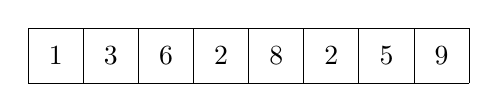
\begin{tikzpicture}[scale=0.7]
\draw (0,0) grid (8,1);
\node at (0.5,0.5) {$1$};
\node at (1.5,0.5) {$3$};
\node at (2.5,0.5) {$6$};
\node at (3.5,0.5) {$2$};
\node at (4.5,0.5) {$8$};
\node at (5.5,0.5) {$2$};
\node at (6.5,0.5) {$5$};
\node at (7.5,0.5) {$9$};
\end{tikzpicture}
\end{center}

まず、次のように分割されます。
\begin{center}
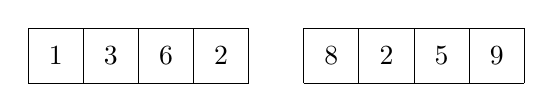
\begin{tikzpicture}[scale=0.7]
\draw (0,0) grid (4,1);
\draw (5,0) grid (9,1);

\node at (0.5,0.5) {$1$};
\node at (1.5,0.5) {$3$};
\node at (2.5,0.5) {$6$};
\node at (3.5,0.5) {$2$};

\node at (5.5,0.5) {$8$};
\node at (6.5,0.5) {$2$};
\node at (7.5,0.5) {$5$};
\node at (8.5,0.5) {$9$};
\end{tikzpicture}
\end{center}

それぞれを次のようにソートします。
\begin{center}
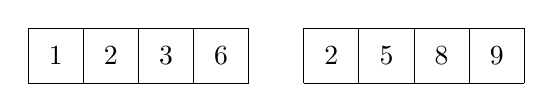
\begin{tikzpicture}[scale=0.7]
\draw (0,0) grid (4,1);
\draw (5,0) grid (9,1);

\node at (0.5,0.5) {$1$};
\node at (1.5,0.5) {$2$};
\node at (2.5,0.5) {$3$};
\node at (3.5,0.5) {$6$};

\node at (5.5,0.5) {$2$};
\node at (6.5,0.5) {$5$};
\node at (7.5,0.5) {$8$};
\node at (8.5,0.5) {$9$};
\end{tikzpicture}
\end{center}

最後にその2つのソートされた配列を結合します。
\begin{center}
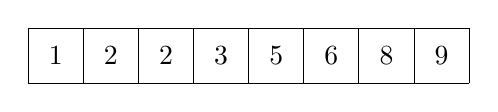
\begin{tikzpicture}[scale=0.7]
\draw (0,0) grid (8,1);
\node at (0.5,0.5) {$1$};
\node at (1.5,0.5) {$2$};
\node at (2.5,0.5) {$2$};
\node at (3.5,0.5) {$3$};
\node at (4.5,0.5) {$5$};
\node at (5.5,0.5) {$6$};
\node at (6.5,0.5) {$8$};
\node at (7.5,0.5) {$9$};
\end{tikzpicture}
\end{center}

\subsubsection{ソート時間の限界 - Sorting lower bound}

ソートの時間を$O(n \log n)$より速くすることは可能でしょうか?
配列要素の比較に基づくソートアルゴリズムに限定すると不可能であることがわかります。

ソートを2つの要素を比較するたびに配列全体の情報が得られる処理とみなし、時間計算量の限界を証明することができます。
この処理を図にすると以下のような木が生成されます。
\begin{center}
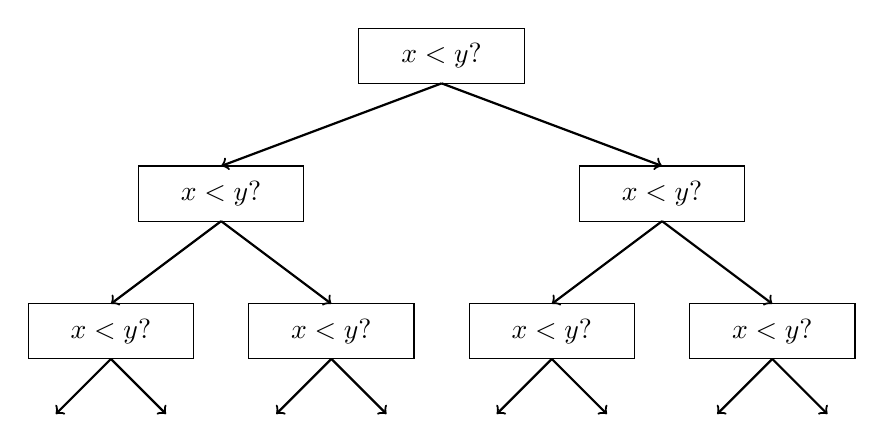
\begin{tikzpicture}[scale=0.7]
\draw (0,0) rectangle (3,1);
\node at (1.5,0.5) {$x < y?$};

\draw[thick,->] (1.5,0) -- (-2.5,-1.5);
\draw[thick,->] (1.5,0) -- (5.5,-1.5);

\draw (-4,-2.5) rectangle (-1,-1.5);
\draw (4,-2.5) rectangle (7,-1.5);
\node at (-2.5,-2) {$x < y?$};
\node at (5.5,-2) {$x < y?$};

\draw[thick,->] (-2.5,-2.5) -- (-4.5,-4);
\draw[thick,->] (-2.5,-2.5) -- (-0.5,-4);
\draw[thick,->] (5.5,-2.5) -- (3.5,-4);
\draw[thick,->] (5.5,-2.5) -- (7.5,-4);

\draw (-6,-5) rectangle (-3,-4);
\draw (-2,-5) rectangle (1,-4);
\draw (2,-5) rectangle (5,-4);
\draw (6,-5) rectangle (9,-4);
\node at (-4.5,-4.5) {$x < y?$};
\node at (-0.5,-4.5) {$x < y?$};
\node at (3.5,-4.5) {$x < y?$};
\node at (7.5,-4.5) {$x < y?$};

\draw[thick,->] (-4.5,-5) -- (-5.5,-6);
\draw[thick,->] (-4.5,-5) -- (-3.5,-6);
\draw[thick,->] (-0.5,-5) -- (0.5,-6);
\draw[thick,->] (-0.5,-5) -- (-1.5,-6);
\draw[thick,->] (3.5,-5) -- (2.5,-6);
\draw[thick,->] (3.5,-5) -- (4.5,-6);
\draw[thick,->] (7.5,-5) -- (6.5,-6);
\draw[thick,->] (7.5,-5) -- (8.5,-6);
\end{tikzpicture}
\end{center}

ここで、''$x<y?$''
とは、ある要素$x$と$y$が比較されることを意味します。
$x < y$ ならば処理は左へ、そうでなければ右へ移動します。
この処理の結果は配列の並べ替えの可能性を示しており、
全部で$n!$のノードからなります。これより、木の高さは少なくとも次の通り示されます。
\[ \log_2(n!) = \log_2(1)+\log_2(2)+\cdots+\log_2(n).\]

最後の$n/2$個の要素を選び、各要素の値を$\log_2(n/2)$に変更することと、
この和の下界を得ることができます。
\[ \log_2(n!) \ge (n/2) \cdot \log_2(n/2),\]
このように、$n \log n$がソートの限界であることが示されました。

\subsubsection{カウントソート - Counting sort}

\index{カウントソート - counting sort}

ソートの計算量の限界が$n \log n$ということを示しましたが、
配列の比較が不要である場合はこの限りではありません。
\key{カウントソート - counting sort} は各要素$c$が
$0 \ldots c$ であることを仮定したソートで、$O(n)$で動作します。

このアルゴリズムは、元の配列を繰り返し処理し、各要素が配列中 に何回現れるかを計算します。
\newpage

\begin{center}
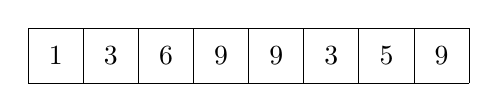
\begin{tikzpicture}[scale=0.7]
\draw (0,0) grid (8,1);
\node at (0.5,0.5) {$1$};
\node at (1.5,0.5) {$3$};
\node at (2.5,0.5) {$6$};
\node at (3.5,0.5) {$9$};
\node at (4.5,0.5) {$9$};
\node at (5.5,0.5) {$3$};
\node at (6.5,0.5) {$5$};
\node at (7.5,0.5) {$9$};
\end{tikzpicture}
\end{center}
この配列の例では出現回数の配列を次のように作ります。
\begin{center}
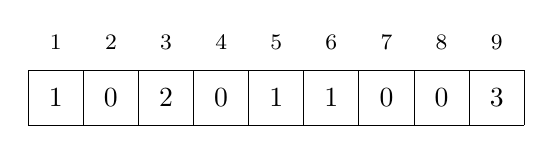
\begin{tikzpicture}[scale=0.7]
\draw (0,0) grid (9,1);
\node at (0.5,0.5) {$1$};
\node at (1.5,0.5) {$0$};
\node at (2.5,0.5) {$2$};
\node at (3.5,0.5) {$0$};
\node at (4.5,0.5) {$1$};
\node at (5.5,0.5) {$1$};
\node at (6.5,0.5) {$0$};
\node at (7.5,0.5) {$0$};
\node at (8.5,0.5) {$3$};

\footnotesize

\node at (0.5,1.5) {$1$};
\node at (1.5,1.5) {$2$};
\node at (2.5,1.5) {$3$};
\node at (3.5,1.5) {$4$};
\node at (4.5,1.5) {$5$};
\node at (5.5,1.5) {$6$};
\node at (6.5,1.5) {$7$};
\node at (7.5,1.5) {$8$};
\node at (8.5,1.5) {$9$};
\end{tikzpicture}
\end{center}

この配列の3の位置の値は2で、要素3が元の配列に2回現れるを意味します。
この構築には$O(n)$の時間がかかり、各要素の出現回数を配列から取得できるため$O(n)$でソート済み配列を作成することができます。
したがって、ソート全体は$O(n)$で動作します。
カウントソートは非常に効率的なアルゴリズムですが定数$c$が十分に小さい場合にのみ使用することができ、
あまりに大きいとカウントの配列を持つことができません。

\section{C++のソート - Sorting in C++}

\index{ソート - sort@\texttt{sort}}

ほぼ全てのプログラミング言語には優れた実装があるので、
自作のソートアルゴリズムをコンテストで使用するのはほとんど良い考えとは言えません。
C++の標準ライブラリには\texttt{sort} という関数があり、
配列などのデータ構造のソートに簡単に利用することができます。

ライブラリ関数を使用することには多くの利点があります。
まず、関数を実装する必要がないため、時間の節約になります。
さらに、ライブラリの実装は正しく効率的です。
自作のソート関数の方が良いということはまずあり得ないでしょう。

C++の \texttt{sort} の使い方をみていきます。
次のコードは配列をソートするものです。
\begin{lstlisting}
vector<int> v = {4,2,5,3,5,8,3};
sort(v.begin(),v.end());
\end{lstlisting}
この処理の後、配列自身が次のように変更されます。
$[2,3,3,4,5,5,8]$となります。
標準では昇順にソートされますが、
つぎのようにすれば降順にできます。
\begin{lstlisting}
sort(v.rbegin(),v.rend());
\end{lstlisting}
vectorでない配列も次のようにソート可能です。
\begin{lstlisting}
int n = 7; // array size
int a[] = {4,2,5,3,5,8,3};
sort(a,a+n);
\end{lstlisting}
\newpage
文字列\texttt{s}をソートすることもできます。
\begin{lstlisting}
string s = "monkey";
sort(s.begin(), s.end());
\end{lstlisting}
これは文字列の各文字をソートすることになり''monkey'' は ''ekmnoy''とソートされます。

\subsubsection{比較演算子 - Comparison operators}

\index{比較演算子 - comparison operator}

\texttt{sort} の関数には
\key{比較演算子 - comparison operator}が定義されていないといけません。
ソートを行う際に2つの要素の比較に常にこの演算子が使用されます。

C++のほとんどのデータ型には比較演算子が組み込まれていて
独自の比較演算関数を用意することなくソートできます。
例えば、数値はその値に従ってソートされ、文字列はアルファベット順にソートされるというようになっています。

\index{pair@\texttt{ペア - pair}}

\texttt{ペア - pair}のソートは、
主に最初の要素(\texttt{first})に従って並び替えられます。
2つのペアの第1要素が等しい場合は、それらは第2要素(\texttt{second})を用いてソートされます。

\begin{lstlisting}
vector<pair<int,int>> v;
v.push_back({1,5});
v.push_back({2,3});
v.push_back({1,2});
sort(v.begin(), v.end());
\end{lstlisting}
この場合は$(1,2)$, $(1,5)$, $(2,3)$と並び替えられます。

\index{tuple@\texttt{タプル - tuple}}

\texttt{タプル - tuple}
も似たようにソートされます。
\footnote{Note that in some older compilers,
the function \texttt{make\_tuple} has to be used to create a tuple instead of
braces (for example, \texttt{make\_tuple(2,1,4)} instead of \texttt{\{2,1,4\}}).}:
\begin{lstlisting}
vector<tuple<int,int,int>> v;
v.push_back({2,1,4});
v.push_back({1,5,3});
v.push_back({2,1,3});
sort(v.begin(), v.end());
\end{lstlisting}
以下のようにソートされます。
$(1,5,3)$, $(2,1,3)$, $(2,1,4)$

\subsubsection{ユーザ定義構造体 - User-defined structs}

ユーザ定義した構造体は比較演算子を定義しなければなりません。
構造体で
\texttt{operator<}を定義する必要があり、
これは引数に同じ型の他の変数を取ります。
小さいと判断する場合に\texttt{true}を、
そうでない場合に\texttt{false}と返すようにします(訳註: 同じ場合はfalseを返すようにします)。

次の構造体\texttt{P}には点のx座標とy座標が格納されています。
比較演算子が定義されているため、この構造体はまずxで比較されて同値ならyで判定されます。

\begin{lstlisting}
struct P {
    int x, y;
    bool operator<(const P &p) {
        if (x != p.x) return x < p.x;
        else return y < p.y;
    }
};
\end{lstlisting}

\subsubsection{比較関数 - Comparison functions}

\index{比較関数 - comparison function}

\texttt{sort}には外部の
\key{比較関数 - comparison function}をコールバック関数として与えることもできます。
次の例では比較関数\texttt{comp}は第一に文字列長で比較し、同点の場合は辞書順で比較するソートを実現します。

\begin{lstlisting}
bool comp(string a, string b) {
    if (a.size() != b.size()) return a.size() < b.size();
    return a < b;
}
\end{lstlisting}
この自作の比較関数を使って次のようにソートすることができます。
\begin{lstlisting}
sort(v.begin(), v.end(), comp);
\end{lstlisting}

\section{二分探索(バイナリサーチ) - Binary search}

\index{二分探索 - binary search}
\index{バイナリサーチ}

配列の要素を検索する最も一般な方法は、\texttt{for} ループを使用することでしょう
たとえば、次のコードは、配列の要素 $x$ を検索します。

\begin{samepage}
\begin{lstlisting}
for (int i = 0; i < n; i++) {
    if (array[i] == x) {
        // x found at index i
    }
}
\end{lstlisting}
\end{samepage}
このコードは最悪の場合で配列の全要素をチェックするので時間計算量は$O(n)$となります。
要素の順序が任意である場合は配列のどこを探せば要素 $x$ が見つかるかという追加情報はないためこの方法は最良の方法です。

ただし、配列がソートされている状況では、より高速に探索を行うことが可能です。
次の\key{二分探索 - binary search}アルゴリズムは,
ソートされた配列の要素を$O(\log n)$で効率的に探索します.

\subsubsection{方法1 - Method 1}

二分探索の通常の実装方法は、辞書の中の単語を探すような作業といえます。
この方法は配列のアクティブな領域を維持します。まず最初はすべての配列要素を含んでいます。
その後、各ステップで領域のサイズを半分にします。

各ステップでは、アクティブな領域の中央の要素を確認します。
中央の要素がターゲット要素であれば、探索は終了します。
そうでない場合は、中央の要素の値に応じて、
領域の左半分または右半分まで再帰的に探索をおこないます。

この実装は以下のようになります。
\begin{lstlisting}
int a = 0, b = n-1;
while (a <= b) {
    int k = (a+b)/2;
    if (array[k] == x) {
        // x found at index k
    }
    if (array[k] > x) b = k-1;
    else a = k+1;
}
\end{lstlisting}

この実装ではアクティブな領域は $a \ldots b$で、
初期値は $0 \ldots n-1$となります。
各ステップで大きさを半分にするため、$O(\log n)$の計算量です。

\subsubsection{方法2 - Method 2}

もう一つの方法は見る配列を効率的にする方法があります。
このアイデアは大きな動きをだんだん小さくしていき、最後に目的の要素を見つけ出します。

探索は配列の左から右へ進めます。最初のジャンプの長さは$n/2$です。
各ステップでジャンプの長さは半分にし、次は $n/4$,
次に $n/8$,$n/16$ .. となり,
最終的に長さは 1 になります。
この結果、目的の要素が見つかったか,配列に現れないことが分かります.

この実装は次のようになります。
\begin{lstlisting}
int k = 0;
for (int b = n/2; b >= 1; b /= 2) {
    while (k+b < n && array[k+b] <= x) k += b;
}
if (array[k] == x) {
    // x found at index k
}
\end{lstlisting}

$b$には今のジャンプの長さが含まれ、これを半分にしていくので計算量は$O(\log n)$です。
\texttt{while}は各ループに対して最大2回呼ばれます。

\subsubsection{C++の標準機能 - C++ functions}

C++標準ライブラリには二分探索ベースのlogで動作する探索の関数が用意されています。

\begin{itemize}
\item \texttt{lower\_bound} $x$以上となる最初の要素へのポインタを返します.
\item \texttt{upper\_bound} $x$よりも大きい最初の要素へのポインタを返します.
\item \texttt{equal\_range} はこの両方へのポインタを返します.
\end{itemize}

これらの関数は配列がソートされていることを前提として動作します。
該当する要素がない場合,ポインタは配列の最後の要素の後を指します.
次のコードは配列の中に値$x$の要素があるかどうかを調べるものです.

\begin{lstlisting}
auto k = lower_bound(array,array+n,x)-array;
if (k < n && array[k] == x) {
    // x found at index k
}
\end{lstlisting}

これらを活用すると次のコードは$x$の数をカウントすることができます。

\begin{lstlisting}
auto a = lower_bound(array, array+n, x);
auto b = upper_bound(array, array+n, x);
cout << b-a << "\n";
\end{lstlisting}

C++では\texttt{equal\_range}という関数によりもっと簡潔に書けます。

\begin{lstlisting}
auto r = equal_range(array, array+n, x);
cout << r.second-r.first << "\n";
\end{lstlisting}

\subsubsection{最小の解 - Finding the smallest solution}

注意するのは、二分探索というのは関数の値が変化する位置を見つけるという点です。
ある問題に対して有効な解となる最小の値$k$を求めたいとします。
$x$が有効な解であれば真を、そうでなければ偽を返す関数$\texttt{ok}(x)$を考えます。
さらに$\texttt{ok}(x)$は$x<k$のとき偽,$x \ge k$の時に真を返すとします。

ここは次のように示せます。
\begin{center}
\begin{tabular}{r|rrrrrrrr}
$x$ & 0 & 1 & $\cdots$ & $k-1$ & $k$ & $k+1$ & $\cdots$ \\
\hline
$\texttt{ok}(x)$ & \texttt{false} & \texttt{false}
& $\cdots$ & \texttt{false} & \texttt{true} & \texttt{true} & $\cdots$ \\
\end{tabular}
\end{center}

\noindent
このような関数がある場合に$k$の値は次のように二分探索で求めることができます。

\begin{lstlisting}
int x = -1;
for (int b = z; b >= 1; b /= 2) {
    while (!ok(x+b)) x += b;
}
int k = x+1;
\end{lstlisting}

この探索は、$\texttt{ok}(x)$ が偽となる最大の値$x$を探索します。
次の値$k=x+1$は、$\texttt{ok}(x)$が真となる最小の値といえます。
ジャンプの長さ$z$の初期値は十分大きくないといけないことに注意してください。
$\texttt{ok}(z)$が真であるような値にしてはならないということです。

アルゴリズムは関数\texttt{ok}を$O(\log z)$ 回呼び出すので、
時間計算量は関数$ok$の計算量に依存します。
たとえば関数が$ O(n)$ 時間で動作するのであれば全体の時間複雑度は$O(n \log z)$となります。

\subsubsection{最大の解の探索 - Finding the maximum value}
二項探索は、まず増加して次に減少する関数の最大値を求める場合にも使用できます。
次のような$k$を見つけたいとします。

\begin{itemize}
\item
$x<k$の時、$f(x)<f(x+1)$
\item
$x \ge k$の時、$f(x)>f(x+1)$
\end{itemize}

これを二分探索で見つけるためのアイデアは $f(x)<f(x+1)$となるような$x$の値を見つけることです。
$k=x+1$であるため、$f(x+1)>f(x+2)$なることを意味します。次のように実装することができます。
\begin{lstlisting}
int x = -1;
for (int b = z; b >= 1; b /= 2) {
    while (f(x+b) < f(x+b+1)) x += b;
}
int k = x+1;
\end{lstlisting}

ここで、連続する値が同値となるケースは動作しないことに注意してください。
同値を引いた時にどちらに探索を続ければいいのかわからないためです。